To classify different types of image sequence we used MLpy library. MLpy is Machine Learning library for python which provides a variety of ML algorithms and tools to perform ML on data.\\
The algorithm used in this project is Linear Support Vector Machine which trained over 5 principle components of the input data produced by previous section.
\subsubsection*{Principle Component Analysis}
Input vector consists of 12 features for every image sequence, 7 HuMoments and 5 Area measures over time. Dataset lies in 12 dimension space. We performed PCA on the input dataset to reduce dimensionality of the original dataset. Prior to Principal Component Analysis we normalize all the features to zero mean and standard deviation. In figure \ref{fig:pcaplot} we can see that only first 5 Principle Components contribute to most variation in the dataset and therefore input data sits on a lower dimension. \\Using these components we project the all the dataset and any other input data into lower 5 dimension subspace.\\

\begin{figure}[htp]
\begin{center}
\leavevmode
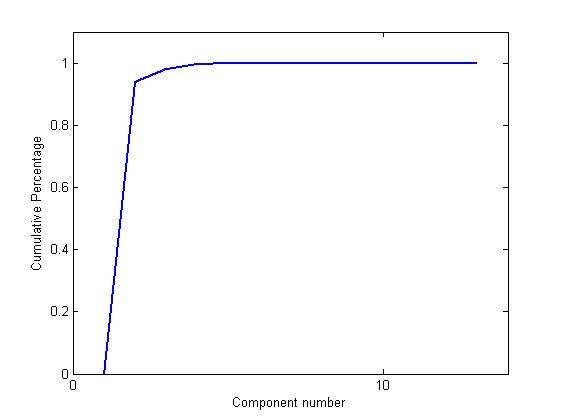
\includegraphics[width=0.6\textwidth] {pca.jpg}
\end{center}
\caption{Cumulative Percentage PCs}
\label{fig:pcaplot}
\end{figure}

\subsubsection*{SVM}
Projected data is then used to train a linear SVM. The algorithm is an implementation of multi-class support vector classification by Crammer and Singer. This algorithm is also available in MLpy library.\\
We also tested Logistic Regression, however as later results will show SVM outperformed. The results for both classifiers are presented in results section.
\subsubsection*{Cross Validation}
In order to evaluate performance of the classifier we utilized Leave-one-out Cross-Validation. The algorithm, at each step takes one instance of data out and performs training on the remaining data and evaluates model on the left out data. Using the trained classifier test instances are checked and results averaged for all dataset.

Summary of the algorithms and parameters used in classification module is presented in table \ref{tbl:classification}.
\begin{table}
\begin{tabular}{|c|l|}
\hline 
Preprocessing: & 1.  Feature Normalization, zero mean standard deviation\\ 
& 2. Principal Component Analysis with 5 Components\\
\hline 
Training Algorithm & Multi-class SVM \\ 
\hline 
Performance Measure & Leave-One-Out Cross-Validation \\ 
\hline 

\end{tabular} 
\caption{Summary of Classification Module parameters and algorithms}
\label{tbl:classification}
\end{table}